\subsection{Instancias}
En general, los sistemas tienen entradas y salidas.  Específicamente los conjuntos de datos entrada y salida pueden ser instancias, atributos y características. Si aterrizamos estos conceptos en una base de datos, las instancias serían las filas. \cite{Aceves2021}

\subsection{Atributos}
Los atributos o registros, corresponden a una instancia particular,  en la matriz de la base de datos son las columnas. Existen distintos tipos de atributos: numéricos, nominales, categóricos ordinales, entre otros.  \cite{Aceves2021}

\subsection{Estadística de atributos}
Cuando se trabaja con datos, es importante saber el tipo de operaciones, cálculos y medidas que nos permiten conocer la tendencia de su comportamiento. A continuación, se describen algunas medidas importantes: 

\begin{itemize}
	\item \textbf{Máximo}: Corresponde al valor más grande contenido en un conjunto de datos o en un atributo.
	\item \textbf{Mínimo}: Corresponde al valor más pequeño contenido en un conjunto de datos o en un atributo.
	\item \textbf{Desviación estándar}: Se define como una medida de la dispersión de un conjunto de datos. A mayor desviación estándar, mayor dispersión de los datos. Su expresión matemática es la siguiente:
	$$s=\sqrt{\frac{\Sigma(x_i-\bar{x})^2}{n-1}}$$
	\item \textbf{Media}: Es una medida de la tendencia central de los datos. Es la suma de los valores de los datos entre la cantidad de datos.
	\item \textbf{Moda}: Dentro de los atributos corresponde al valor  que más se repite dentro de los atributos.
\end{itemize}

\subsection{Tipo de distribución}
El histograma permite conocer el tipo de distribución de los datos con los que se trabajará, existen distintos tipo de distribución, dentro de los cuales se puede destacar \cite{Aceves2021}:

\begin{itemize}
	\item \textbf{Uniforme}: Mostrada en Figura \ref{Fig: DistUni}.
	\item \textbf{Normal (unimodal)}: Mostrada en Figura \ref{Fig: DistNor}.
	\item \textbf{Unimodal sesgada izquierda}: Mostrada en Figura \ref{Fig: DistSIz}.
	\item \textbf{Unimodal sesgada derecha}: Mostrada en Figura \ref{Fig: DistSDe}.
	\item \textbf{Multimodal}: Mostrada en Figura \ref{Fig: DistMul}.
\end{itemize}

\begin{figure}[htbp]
	\centering
	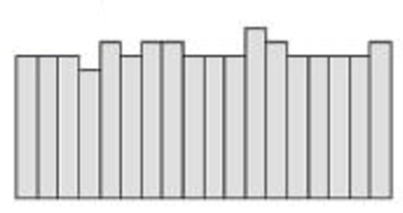
\includegraphics[width=0.25\textwidth]{DistribucionUniforme}
	\caption{Ejemplo de distribución uniforme.}
	\label{Fig: DistUni}
\end{figure}

\begin{figure}[htbp]
	\centering
	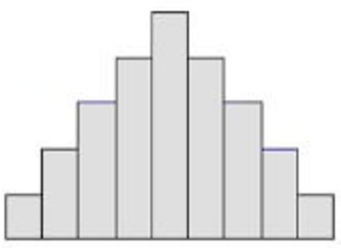
\includegraphics[width=0.25\textwidth]{DistribucionNormal}
	\caption{Ejemplo de distribución normal.}
	\label{Fig: DistNor}
\end{figure}

\begin{figure}[htbp]
	\centering
	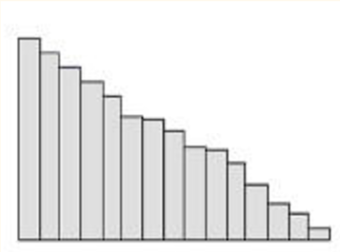
\includegraphics[width=0.25\textwidth]{DistribucionSesgadaIzq}
	\caption{Ejemplo de distribución sesgada a la izquierda.}
	\label{Fig: DistSIz}
\end{figure}

\begin{figure}[htbp]
	\centering
	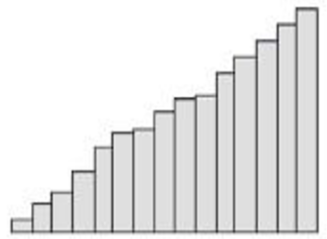
\includegraphics[width=0.25\textwidth]{DistribucionSesgadaDer}
	\caption{Ejemplo de distribución sesgada a la derecha.}
	\label{Fig: DistSDe}
\end{figure}

\begin{figure}[htbp]
	\centering
	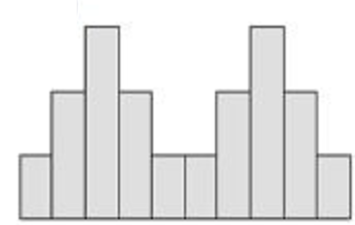
\includegraphics[width=0.25\textwidth]{DistribucionMultiModal}
	\caption{Ejemplo de distribución multimodal.}
	\label{Fig: DistMul}
\end{figure}

\subsection{Relaciones entre atributos}
\begin{itemize}
	\item \textbf{Cuartiles}: Se definen como los valores que dividen un conjunto de datos en cuatro subconjuntos que poseen alrededor del mismo número de observaciones. El total de los datos corresponde al 100\%, y este se divide en 25\%, 50\%, 75\% y 100\%. \cite{Economipedia}
	\item \textbf{Varianza}: Es la medida de dispersión de los datos con respecto a la media de los mismos. \cite{IAnet20201}
	\item \textbf{Covarianza}: Mide la variabilidad entre dos variables. Su valor será positivo si las variables si la relación entre ellas es lineal y van en la misma dirección, en cambio, será negativa si su relación es inversa. \cite{IAnet20202}
\end{itemize}

\subsection{Datos atípicos en atributos}
Resulta importante conocer la calidad de los datos con los que se trabajará, y los problemas que este pueda presentar por su naturaleza misma. Existen problemas como valores faltantes, problemas con la cardinalidad irregular y valores atípicos. \cite{Aceves2021}

Particularmente los valores atípicos son aquellos que están muy alejados de la tendencia central. Pueden ser causa de errores cuando el registro de los datos se genera de manera manual o puede suceder cuando realmente un valor está muy alejado del resto, debido al tipo de información que se está registrando. \cite{Aceves2021}
